	\documentclass[conference]{IEEEtran}
\usepackage{amsmath}
\usepackage[spanish]{babel} %Definir idioma español
\usepackage[sort&compress]{natbib}
\usepackage[utf8]{inputenc} %Codificacion utf-8

\usepackage{graphicx}



\begin{document}


\title{Narración Interactiva: \\
Un enfoque aplicando la personalidad y el comportamiento del jugador en el desarrollo de la historia.}


% author names and affiliations
% use a multiple column layout for up to three different
% affiliations
\author{\IEEEauthorblockN{José David Mamani Vilca}
\IEEEauthorblockA{Ciencia de la Computación \\ Universidad Católica San Pablo \\ Email: jose.mamani.vilca@ucsp.edu.pe}
}

% make the title area
\maketitle

\begin{abstract}

Contar historias es una capacidad innata en los seres humanos. Esta habilidad para organizar conocimientos y compartir  experiencias recibe el nombre de Inteligencia Narrativa. Con los avances en la Industria de los Videojuegos y la Inteligencia Artificial se ha hecho posible extender dicha habilidad a las computadoras. En la presente investigación analizaremos un campo dentro de la Narración Interactiva. Basados en un sistema propuesto por Soares de Lima \citep{de2018player}, implementaremos un juego capaz de adaptar sus mecánicas y líneas narrativas a el comportamiento y personalidad del jugador. 

\end{abstract}

% no keywords

\begin{IEEEkeywords} Narración Interactiva, Player Modeling, Personality, Quest Generation, Games, Artificial Intellegence\end{IEEEkeywords}


% For peer review papers, you can put extra information on the cover
% page as needed:
% \ifCLASSOPTIONpeerreview
% \begin{center} \bfseries EDICS Category: 3-BBND \end{center}
% \fi
%
% For peerreview papers, this IEEEtran command inserts a page break and
% creates the second title. It will be ignored for other modes.
\IEEEpeerreviewmaketitle

\section{Introducción}

La narración de historias dentro de un videojuego difiere en gran medida de la narracion tradicional (Cuentos, Novelas, Películas, Canciones, etc). Cada vez que narramos una historia nos proponemos el compartir diferentes experiencias con otros ordenando una serie de sucesos de forma inteligente y atractiva. Este mismo proceso es estándar para cada casi todo ambiente siendo la única excepción aquellos que postulan la opción de interectividad.  Una historia interactiva es aquella que posee la cualidad de modificarse y adaptarse a las elecciones del receptor. Los videojuegos poseen casi en su totalidad la cumbre de esta interactividad.

La Narración Interactiva se entiende como un modelo que empuja al jugador a realizar acciones que modifican el contexto narrativo en un juego. Esta característica narrativa esquiva el diseño linear basado en misiones de juegos como \textit{Mass effect 2} o \textit{Mafia 2 }  mejorando la inmersión del usuario al darle importancia a sus decisiones  y a sus acciones ( \textit{The Walking Dead: The Final Season}, \textit{The Elder Scrolls: Skyrim}, ...). Esta característica sencilla de entender presenta, sin embargo, una serie de dificultades consecuentes a el grado de libertad que se le da a el usuario. Mantener la coherencia de la historia, por ejemplo, o implementar líneas narrativas secundarias como consecuencia de acciones imprevistas son solo algunas de las dificultades a resolverse en caso incorporar este modelo en un juego. 

En el presente trabajo desarrollamos una investigación en torno a la narración interactiva el cuál aplicado en un videojuego, es capaz de adaptarlo a distintas líneas narrativas acorde a modelos de comportamiento y personalidad previamente obtenidos. Esta técnica mejora en gran medida la percepción de inmersión pues altera las mecánicas del juego, valora la actitud del jugador durante la toma de decisiones y añade un factor de dinamicidad al desenvolvimiento del juego en general.

\section{Trabajos Relacionados}

Diversas investigaciones han sido presentados para analizar y profundizar en las distintas actitudes que un jugador puede tomar dentro de un juego. Uno de los modelos más tempranos fue el presentado por Richard Bartle \citep{bartle1996hearts} en el año 1996, en donde se clasificaba a los jugadores en torno a cuatro grupos: Aquellos centrados en completar una misión, los sociables,  los exploradores y los asesinos. Otra clasifación derivada de esta fue la presentada por Bateman y Bonn \citep{bateman200521st} en donde los jugadores eran clasificados en base a cuatro indicadores de personalidad: los Conquistadores, los gestores, los vagabundos y los participantes. Estos indicadores tomaban por referencia los tres aspectos sociales que motivaban la actitud de un jugador: Sus logros, su entorno social y el nivel de inmersión que buscaban. Un tercer modelo, esta vez basado en la campo neurobiologico, fue presentado por Nacke \citep{nacke2014brainhex}, en donde se diferencian siete arquetipos de jugador: Los buscadores, los supervivientes, los temerarios, los manipuladores, los consquistadores, los sociables y los \textit{quest finder}. Sin embargo, todos estos modelos presentan la problemática de definir un tipo estático de jugador, razón por la cuál no se ajustan de forma muy eficiente a la realidad de la personalidad y el comportamiento humano. 	

Derivada de esta problemática diversas implementaciones surgieron para considerar el factor de personalidad humana en las mecánicas de un juego. Por ejemplo, Missura y Gärtner \citep{missura2009player} propusieron un modelo utilizado en juegos del género \textit{First Person Shooter} para adaptar la mecánicas el mismo en torno a factores tales como: Experiencia del jugador, balance del juego, generación de contenido apoyado en parámetros de personalidad, etc. Estas características eran recopiladas mediante el uso de vectores de personalidad que reflejaban los comportamientos que el jugador mostraba y que posteriormente se recopilarían en un modelo más estandarizado. Por otro lado, Weber y Mateas \citep{weber2009data} propusieron un algoritmo de clasificación de jugadores en torno a las estrategias que estos seguían. Dicho modelo fue utilizado en el juego \textit{StartCraft} y permitía modificar el balance y nivel de dificultad en torno al desempeño de cada jugador. Una tercera implementación fue propuesta Spronck y Den Teuling \citep{spronck2010player} para contruir un modelo del jugador en torno a las preferencias del mismo utilizando un clasificador SMO (\textit{Sequential Minimal Optimization}).

Obtenidos los modelos de personalidad humana, las propuestas de interactividad en videojuegos se centraron en el \textit{Story Telling}. Baber y Kudenko \citep{barber2007user} propusieron un modelo capaz de generar historias de forma interactivad considerando vectores de personalidad que se iban modificando conforme el algoritmo detectaba rasgos en el jugador que influían de forma directa en el desarrollo de la historia. Otro modelo muy conocido fue \textit{Miracle}, propuesto por Seif El-Nasr \citep{el2007interaction}, el donde el sistema de interactividad  a nivel del \textit{StoryTelling} se apoyaba no solo en modelos de personalidad sino en modelos de comportamiento humano. Puede considerarse a este último modelo como uno de los más completos pues el índice de inmersión que el jugador experimentaba era mucho mayor que en implementaciones previas.  Finalmente el tercer modelo es pASSAGE, propuesto por Thue et al. \citep{thue2007interactive}. Este modelo comparte muchas similutes con el modelo previo con la diferencia de que el reconocimiento de los modelos de comportamientos se realiza de forma regular y siempre considerando los datos que el jugador deja en el juego. 



\section{Narración Interactiva}

\subsection{Sistema de Planeamiento}

\subsubsection{Misiones por Jerarquía}

La jerarquía dentro de la historia de un videojuego deriva en el uso de \textit{quest} o misiones. Cada misión en sí representa una pequeña porción de la historia y generalmente poseen un inicio y un final que dependen o hacen depender a otras misiones. Las misiones pueden a su vez estar divididas en varias otras que dependiendo de su resultado pueden afectar la conclusión de la misión \textit{padre}. Esto implica que cada misión pueda poseer múltiples estados en donde se pueda señalar el progreso de la misión principal, las decisiones que el jugador optó por tomar y las posibles variaciones que se pueden realizar en la historia. Esta última característica, además, es fundamental si se desea añadir el factor dinamicidad a la historia, pues 
acorde a los datos adquiridos del jugador, podemos definir un comportamiento no determinístico en la generación de historias.

Otro concepto fundamental dentro de los \textit{quest} es el término \textit{event} el cuál permite describir un escenario en particular dentro del juego que debe alcanzarse para disparar una serie de acciones  como respuesta a ese estado. Un ejemplo muy común se da cuando se alcanza un determinado lugar del mapa y se active un evento que permita la generación masiva de enemigos \textit{Left 4 Dead} o la aparición de un enemigo en particular \textit{Half Life, House of the Dead, etc}. Los eventos también pueden ser utilizados para describir estados del jugador, ya sea en su personalidad, en su comportamiento o en su desempeño dentro del juego.

\subsubsection{Arquitectura del sistema}

Basado en el modelo presentado por \citep{de2018player} podemos describir el sistema en ocho módulos importantes:

\textit{Quest Planner} es el encargado de definir un orden lógico para alcanzar la completitud de una misión. \textit{Quest Monitor} verifica si el orden de los sucesos va acorde a el desempeño del jugador y lo descrito en el sistema, \textit{Quest Manager} queda a cargo de administrar múltiples intancias de los módulos presentados previamente (Cabe resaltar que la gran mayoría de juegos, dependiendo de su género, son capaces de manejar diversas misiones al mismo tiempo) y \textit{Quest Library} es el encargado de mantener y administrar una base de datos con toda las \textit{quest} y  \textit{sub quest} disponibles. Finalmente, \textit{Game Manager} es capaz de modificar el estado actual del juego acorde a los resultados obtenidos por los módulos previos.

Por otro lado, los módulos restantes, \textit{World State}, \textit{Player Model} y \textit{Players Assistant} desempeñan labores más externas en el manejo de los \textit{quests}. \textit{World State} es un módulo encargado de administrar los efectos producidos por los \textit{quests} dentro del mundo siendo en algunos casos dependiente del  \textit{Game Manager} para recopilar la información necesaria. Por su parte, \textit{Player Model} es un módulo encargado de definir la personalidad y el comportamiento dentro del juego del jugador. Cabe resaltar que estos dos últimos conceptos son completamente distintos siendo la personalidad un estado inicial del jugador dentro del juego mientras que el comportamiento está relacionado con el desempeño que el jugador tiene durante el mismo. Por último \textit{Players Assistant} es un módulo más secundario encargado de asesorar al jugador durante el desarrollo de los \textit{quests}.


\begin{figure}[tph!]
\centerline{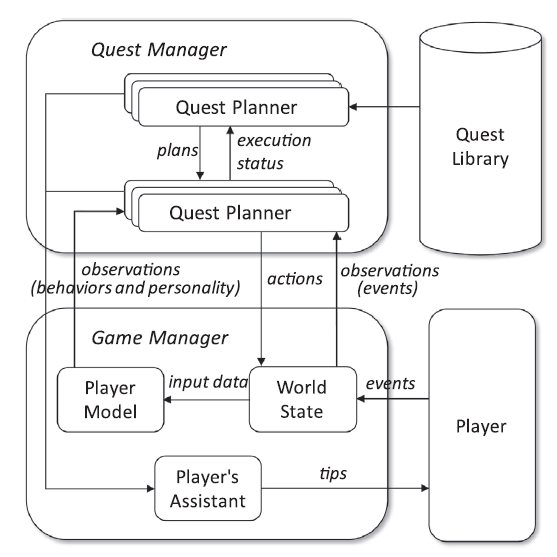
\includegraphics[totalheight=8cm]{1}}
    \caption{Arquitectura del Sistema}
    \label{fig:red1}
\end{figure}

\subsection{Modelo de Comportamiento para el Jugador }

Como se mencionó previamente, es importante recalcar la diferencia entre el comportamiento y la personalidad de un jugador. El comportamiento humano es el resultado de complejos procesos reflexivo-impulsivos \citep{strack2004reflective}. Además es totalmente dinámico , varía con el paso del tiempo acorde a una situación y bajo un contexto \citep{mishra2008psychology}. Esto deriva en que el modelo orientado a reconocer el comportamiento de un jugador debe ser capaz de reconocer el factor dinámico presente en la naturaleza del mismo.

Un enfoque inicial para dicho modelo se da en la imagen \ref{fig:red2}, en donde se describe un sistema con tres componentes principales: El componente de entrada, el componente de salida y la función de comportamiento . 

\begin{figure}[tph!]
\centerline{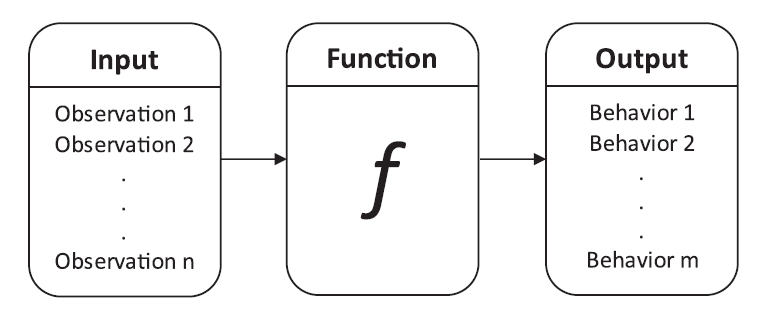
\includegraphics[totalheight=3cm]{2}}
    \caption{Modelo de Comportamiento}
    \label{fig:red2}
\end{figure}

\medskip
\subsubsection{Componente de Entrada (Observación)}

Como su nombre lo describe, el componente de entrada es el encargado de observar al jugador a lo largo de todo el juego. Durante dicho proceso este componente recolecta datos relacionados a las características principales del mismo. Por ejemplo; aplicado bajo un juego del tipo \textit{First Person Shooter} los datos más importantes a recolectar serían aquellos  relacionados  con las estadísticas de los disparos (Puntería, número de balas, tiempo entre disparos, etc), o en el caso de un juego \textit{SandBox} resaltaría características tales como terreno explorado, tiempo entre misiones o relación con NPCs. Estas características en su mayoría suelen ser únicas para un tipo de videojuego, pero tampoco podemos descartar la existencia de característcas globales y aplicables para cualquier género. Por otro lado, definir este conjunto de datos iniciales es de suma importancia pues una selección erronéa conduciría a patrones de respuestas inadecuados para un género de videojuego.


Otro factor a destacar en este componente es la frecuencia con la que los datos del jugador son recolectados. Este modelo no propone evaluar los datos del jugador de forma continúa, sino bajo un determinado intervalo de tiempo (\textit{Time Windows}). El lapso que tomaría evaluar y posteriormente entregar los datos para ser analizados es crucial (Tanto o incluso más que las características definidas inicialmente). Un lapso de tiempo muy corto resultaría ser inútil, pues el conjunto de datos a analizar no entregaría la información necesaria para poder definir un modelo de comportamiento para ese instante. Por otra parte, un lapso de tiempo muy largo resultaría poco conveniente, pues este sería incapaz de detectar la naturaleza dinámica del comportamiento. Bajo esta última posibilidad, los datos obtenidos serían incapaces de representar la transición entre dos estados del jugador por lo que la información final sería en el peor de los casos, totalmente erronea. Otro punto a destacar bajo este último factor, y que además no se analiza en esta propuesta, es definir una naturaleza dinámica para la  frecuencia misma con la que los datos son recolectados.  

\medskip
\subsubsection{Componente de Salida (Comportamiento)}
El componente de salida es el encargado de establecer todos los posibles modelos de pesonalidad que el juego puede definir para un jugador a modo de comportamiento. Estos modelos se obtienen tras haber analizado los datos recolectados por el componente previo y predicen que comportamiento se desenvolverá más adelante y que acciones deben realizarse dentro del juego para poder contrarrestarlos. 

Una característica sumamente importante en estos modelos, es la capacidad ampliamente descriptiva que deben poseer para lograr abarcar cada aspecto en el comportamiento de un jugador. Una forma muy común de definir estos modelos (y muy extendida en implementaciones previas de \textit{Player Modeling}) es mediante el uso de arquetipos de personalidad \citep{tuunanen2012meta}. Esta técnica si bien permite abarcar de forma rápida a la mayoría de jugadores, presenta deficiencias al momento de establecer características específicas dentro de un modelo. Un ejemplo claro se da en aquellos jugadores que presentan una personalidad sumamente variada, capaz de contener simultáneamente distintos modelos definidos dentro del sistema.

Para lograr describir con mayor detalles los aspectos de estos modelos, se utiliza una teoría ampliamente aceptada dentro de la personalidad humana: \textit{The Five Factor Model} o  \textit{The Big Five} \citep{goldberg1990alternative}.\textit{The Big Five} está compuesto por una serie estructurada de rasgos en la personalidad humana, las cuales en conjunto, son capaces de representar la gran diversidad de modelos de personalidad que existen. 

\textit{The Big Five está compuesto por cinco factores:}

\begin{itemize}
\item \textbf{Openness: } Aquellos que destacan  por ser curiosos, imaginativos y abiertos a nuevas experiencias. Los que presentan un bajo puntaje en este factor suelen ser indiferentes y poco interesados.

\item \textbf{Conscientiousness: } Describe a aquellos con personalidades meticulosas, capaces de analizar una situación de forma prolongada y bastantes  cautos al momento de hacer una elección. Por el contrario, aquellos con poco puntuación en este rasgo, suelen ser más desordenados, capaces de enfrentar situaciones inesperadas y con poco interés en planear estrategias.

\item \textbf{\textit{Extraversion}: } Un alto puntaje en este rasgo describe a las personas con altas habilidades sociales, capacidades de socialización exepcionales y mucho interés en establecer vínculos nuevos. Un puntajes bajo, en cambio, engloba a  las personas tímidas, con poco interés en la socialización y ciertamente cerrados a relacionarse con nuevos individuos. 

\item \textbf{\textit{Agreeableness}: } Representa a las personas con mucha iniciativa en el trabajo cooperativo, de personalidad amigable y completamente inclinados a prestar ayuda durante situaciones difícles.  Su contraparte, en cambio, encierra aquellos de naturaleza hostil, con poco o nulo interés en la situación ajena y completamente enfocados en su bienestar personal. 

\item \textbf{\textit{Neuroticism}: } De todos los rasgos, este suele ser el que mejor se logra identificar. Aquellos con altos puntajes se describen como personas  emocionalmente inestables, incapaces de llevar una situación de forma controlada y con alta tendencia a reaccionar de forma agresiva. Su contraparte, por otro lado, destaca por ser un individuon calmado, capaz de pensar y analizar una situación sin llegar a los límites del estrés.

\end{itemize}

Como se pudo intuir, \textit{The Big Five} funciona bajo un sistema de puntaje y aproximación. La evaluación de estos rasgos se realiza por medio de tests o cuestionarios que dependiendo de las respuestas, inclinan los parámetros de personalidad hacia aquellos rasgos que mejor los describen.  Esto deriva en la ventaja de no necesitar modelos de personalidad predefinidos que engloben las acciones de un jugador, además de que todos los posibles resultados describen con mejor eficiencia al usuario.

\begin{figure}[tph!]
\centerline{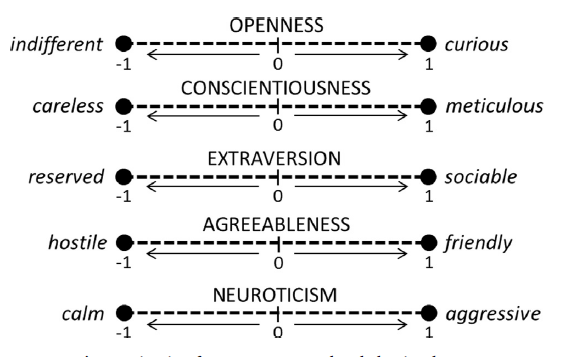
\includegraphics[totalheight=5cm]{3}}
    \caption{\textit{The Big Five} representado en axis de aproximación}
    \label{fig:red3}
\end{figure}

Si bien hasta este punto consideramos a \textit{The Big Five} como una forma eficiente de describir un modelo de personalidad, también podemos utilizarlo para describir un modelo de comportamiento. De hecho las fuentes de esta investigación señalan las pruebas hechas por Back \citep{back2009predicting} con base en \textit{The Big Five} para describir modelos comportamiento tomando por base  modelos de personalidad. Estas evaluaciones permitieron asociar los comportamientos de un jugador con cualquiera de los  cinco rasgos descritos por \textit{The Big Five}. Por ejemplo: Un jugador curioso e interesado demostaría en el juego un comportamiento altamente dinámico, con tendencias a la exploración y búsqueda de nuevas misiones. Este comportamiento también se vería reflejado en los rasgos de \textit{Big Five}, siendo \textit{Openness} el rasgo con mayor puntuación, a la vez que \textit{Conscientioness} sería el de menor. Algunos comportamientos que podemos englobar con \textit{The Big Five} se presentan a continuación:

\begin{itemize}
\item[•] $F_1$ Procentaje del tiempo en el que el jugador está detenido.
\item[•] $F_2$ Porcentaje del tiempo en el que el jugador está caminando.
\item[•] $F_3$ Porcentaje del tiempo en el que el jugador está colisionando.
\item[•] $F_4$ Total de áreas exploradas.
\item[•] $F_5$ Total de disparos en cada \textit{Time Window}.
\item[•] $F_6$ Porcentaje de disparos acertados.
\item[•] $F_7$ Porcentaje de disparos fallados.
\item[•] $F_8$ Porcentaje de enemigos eliminados.
\item[•] $F_9$ Tiempo ponderado entre cada disparo del jugador.
\item[•] $F_10$ Distancia promedio en la cuál los enemigos fueron eliminados.
\item[•] $F_11$ Distancia promedio en la cuál el jugador les disparo a los enemigos.
\item[•] $F_12$ Tiempo promedio en el cual el jugador vio al enemigo y lo eliminó
\item[•] $F_13$ Porcentaje de kits médico recogidos por el jugador
\item[•] $F_14$ Porcentaje de vida que el jugador a recuperado sin propósito alguno.
\item[•] $F_15$ Tiempo promedio en el cuál el jugador vió un kit médico y lo recogió.
\item[•] $F_16$ Porcentaje de munición recogida.
\item[•] $F_17$ Tiempo promedio en el cuál el jugador vió un paquete de munición y lo recogió.
\item[•] $F_18$ Porcentaje de NPCs con los cuáles el jugador se ha relacionado.
\item[•] $F_19$ Tiempo promedio en el cuál el jugador vió un NPCs e interactuó con él.
\item[•] $F_20$ Porcentaje de NPCs rescatados por el jugador.
\item[•] $F_21$ Tiempo promedio en el cuál el jugador vió un NPC en peligro y lo rescató.
\item[•] $F_22$ Daño total sufrido en cada \textit{Time Window}.
\item[•] $F_23$ Número de cambio de direcciones que el jugador ha realizado en un \textit{Time Window}.

\end{itemize}

Los resultados de este componente estarían completamente enfocados a modificar los cinco rasgos de \textit{The Big Five}, cada uno de ellos entre los rangos de $[-1, 1]$, variando dinámicamente acorde a los datos recogidos en cada \textit{Time Windows}.

\medskip
\subsubsection{Función para el reconocimento del comportamiento.}

Descritos los componentes de entrada y salida se hace necesario definir la función que traduce los datos recogidos en cada \textit{Time Window} a comportamientos descritos para nuestro juego (La componente de salida que utilizará el modelo de comportamiento). 

Tomando por base la naturaleza de nuestro sistema, un problema de Regresión con Salida Múltiple, resulta conveniente el uso de una Red Neuronal Artificial. Los rasgos establecidos dentro de \textit{The Big Five} son cinco, e irán obteniéndose conforme el jugador se desenvuelve dentro del videojuego, por lo que representan un escenario más que ideal para la aplicación de este sistema.

Entrenada correctamente, la Red Neuronal debe ser capaz de predecir comportamientos en torno a patrones previamente establecidos (de ahí que sea crucial una correcta definición de estos). Sin embargo, su uso también conlleva riesgos de rendimiento pues esta función depende del margen de tiempo en la que se actualiza y que por ende consume más recursos (Este problema se analizará con mayor profundidad dentro de la etapa de Experimentación).

Para nuestra implementación actual se hará uso de una Red Neuronal del tipo \textit{Single Hidden Layer} compuesta de 64 neuronas y que utilice una función sigmoidal. El algoritmo se desarrollará usando la implementación hecha en la librería FANN para posteriormente pasar por sesiones de aprendizaje en donde se definirán todos los posibles patrones de comportamiento a reconocer. 	

\subsection{Modelo de Personalidad para el Jugador}

A estas alturas ya debemos ser capaces de discernir entre Comportamiento y Personalidad.  El primero es de naturaleza cambiante, en relación al contexto, al lugar y a la interacción. El segundo es más estático, imperceptible para su poseedor pero notable para sus compañeros. Una definición súmamente concluyente es la dada por Costa y McCrae \citep{mccrae1997personality} \textit{La personalidad se define como la combinación de características que distinguen a un personaje, que resalta su forma de pensar, sus pensamientos y sus acciones}. Básicamente la personalidad define al ser (al menos en un plano superficial) y de esta surgen la mayoría de comportamientos.

Podemos definir la personalidad de nuestro jugador mediante el uso de cuestionarios o exámenes que evalúen los cinco rasgos del personalidad que vimos en \textit{The Big Five}. Sin embargo, el modelo de personalidad tiene peculiaridades que debemos considerar al momento de establecerlo. Debido a su naturaleza estática solo es necesario definirlo durante las etapas iniciales del juego. También es importante hacerlo sin ningún tipo de influencias pues lo que se busca es construir un modelo de personaliad orientado a la actitud real del jugador y no a la que se reflejaría  dentro del mundo virtual. Tampoco podemos descartar la idea de alterarlo ligeramente con cada sesión de juego, pues el jugador no siempre mantendrá la misma personalidad durante intervalos de tiempo muy largos (de semanas a meses).

\subsubsection{Estrategias para la captación de la personalidad.}

El uso de cuestionarios y tests se presentan como los mejores métodos para construir un modelo de personalidad, pero cargan con la desventaja de ser poco apropiados para un entorno como lo es el de los videojuegos. Si ir más lejos, un modelo de personalidad basado en \textit{The Big Five} requiere de al menos 44 preguntas y en ciertos casos de hasta 128 para poder establecerse. Resolver semejante cantidad de preguntas resulta totalmente impráctico (Especialmente para los \textit{gamers} con ritmos de vida muy ajustados de tiempo). Debido a esto se hace necesario el uso de cuestionarios con versiones más resumidas de \textit{The Big Five}: BF-10 \citep{rammstedt2007measuring}.

BF-10(\textit{Big Five Ten}) es un cuestionario de 10 preguntas con la ventaja de poder resolverse de forma muy rápida. Entre las características que lo hacen más apropiado resalta el hecho de ofrecer resultados por escala (entre 1-5). Sus preguntas están diseñadas con el propósito de representar los 2 extremos de un rasgo de comportamientos además de ser psicologicamente más exactas. BF-10 ofrece preguntas en torno a los siguiente factores:

\begin{itemize}
\item (1) Me veo a mí mismo como alguien reservado...
\item (2) Me veo a mí mismo como alguien capaz de confiar en otros...
\item (3) Me veo a mí mismo como alguien con tendencia a la vagancia...
\item (4) Me veo a mí mismo como alguien relajado, capaz de manejar situaciones estrés...
\item (5) Me veo a mí mismo como alguien de interese artísticos...
\item (6) Me veo a mí mismo como alguien sociable...
\item (7) Me veo a mí mismo como alguien que distingue mucho los defectos ajenos...
\item (8) Me veo a mí mismo como alguien capaz hacer un trabajo de buena manera...
\item (9) Me veo a mí mismo como alguien muy nervioso...
\item (10) Me veo a mí mismo como alguien de mucha imaginación...
 
\end{itemize}

Devolviendo resultados con rangos de aceptación:

\begin{itemize}
\item (1) Totalmente en desacuerdo.
\item (2) Ligeramente en desacuerdo.
\item (3) Ni de acuerdo o desacuerdo.
\item (4) Ligeremente de acuerdo.
\item (5) Totalmente de acuerdo.
\end{itemize}

La preguntas relacionadas en torno a un rasgo de la personalidad posteriormente se ponderan y se obtienen los valores exactos para cada rasgo de \textit{The Big Five}.

Utilizar directamente BF-10 dentro de nuestro juego aún resulta inviable pues requiere de la participación directa del jugador para identificar su personalidad (Cosa que raramente consigueremos). El problema de la implementación hasta este punto es que va contra los principios de inmersión que un juego necesita mantener para no perder la atención del jugador. Una buena forma de resolver este problema es adaptando BF-10 al contexto en donde vamos a utilzarlo. Para lograrlo haremos uso de escenas relacionadas a la historia que el juego planea. Durante el transcurso de cada escena se plantea una problemática que el jugador debe responder y que posteriormente será utilizada como resultados en una da las preguntas de BF-10. De esta manera evitamos arruinar la experiencia del jugador y al mismo tiempo recolectamos los datos que necesitamos. 


\subsection{Planeamiento de historia}

Las \textit{quest} o misiones están entre los factores cruciales que definen cuán interesante puede llegar a ser un juego. Si bien, las líneas narrativas de nuestra historia ya están definidas desde un principio, el desarrollo de los \textit{quest} que las componen aún pueden presentar un comportamiento más dinámico.

Como vimos previamente, el \textit{Quest Planner} será el encargado de estructurar las misiones. Un \textit{Quest} puede describirse en la siguiente tupla:

$$Q = (P, S_0, G, H)$$

\begin{itemize}
\item  En donde $P$ representa a un conjunto de expresiones bajo la forma $(r_1, ..., r_k)$ , siendo cada $r_i$ un predicado que describe términos distintos (desde variables \textit{H1, T1} hasta palabras simples \textit{JUGADOR} o \textit{MEDICINA}).

\item $S$ es un subconjunto de $P$.

\item $G$ como conjunto de objetivos $G = {G_1, G_2 ...}$ descritos a su vez dentro de $P$. Los objetivos pueden tener el siguiente formato: $G1 = {dead(enemie)}, G2 = {have(key)}, G3 = go{next level}$ y acorde a su disposición, guían el desenvolvimiento de una misión. 



\item $H$ como un par compuesto por $(C_i, T_i)$ que puede ser leído como \" Si $C_i$ entonces $T_i$ \". $C_i$ es utilizado como un valor de comparación que indica el grado necesario en un rasgo de la personalidad para poder  ser verdadero. (\textit{Si 0.37 en Openess, entonces...}). Por otro lado, $T_i$ representa al conjunto de objetivos descritos en $G$ pero ordenados de tal forma que exista codependiencia entre ellos, por ejemplo: Siendo $T_i$ y $T_j$ dos objetivos del \textit{quest} y además $ i < j $, entonces el objetivo $T_j$ no podrá alcanzarse sin antes completar $T_i$. Este par compuesto resulta ser sumamente importante, pues define la condiciones necesarias para desplegar cada posible linea narrativa en relación a la personalidad. Por ejemplo, considerando los objetivos $G_1, G_2, G_3$ del item previo, $C1 = {agreeableness >= 0.4, conscientiousness > 0.8}$ y $T1 = {G_2, G_1, G_3}$, podemos entender que si el jugador cumple con la condición de $C1$ podrá acceder a la secuencia de narración $T1$ conformada por los objetivos desplegados en  orden $G_1, G_2, G_3$.
 
	
\end{itemize}


\begin{figure}[tph!]
\centerline{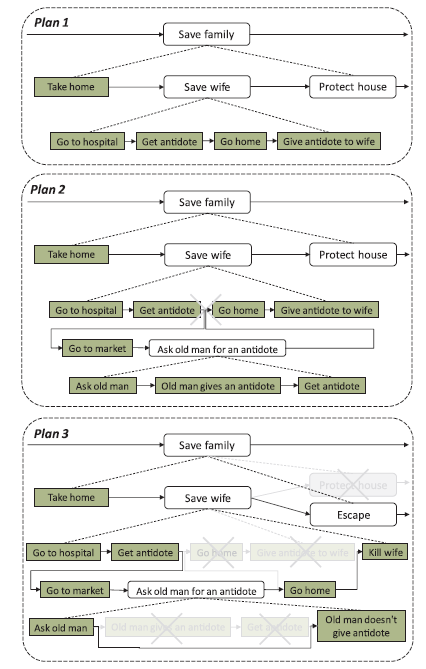
\includegraphics[totalheight=12cm]{7}}
    \caption{ \textit{Quest} con diversos planes de ejecucición. }
\end{figure}

\medskip
\subsection{Experimentación}
Con el propósito de validar la interactividad bajo ambas propuestas se procedió con la implementación de un videojuego del género \textit{Run and Gun} (un género similar al presentado en \textit{Contra}). El videojuego de título \textit{Nightmare} comprende la historia de Elizabeth, una joven envuelta en un mundo de sueños derivados de sus problemas en la vida real. Elizabeth deberá explorar hasta el ambiente más recóndito dentro de su cabeza para poder finalmente escapar de aquél mundo residual que la absorbe y que poco a poco va tornándose más pesallidezco.

\textit{Nightmare} es un prototipo orientado a la alta interactividad basándose en los comportamientos registrados del jugador. El sistema es capaz de generar diversas líneas narrativas derivadas de las carácteristicas relacionadas con \textit{Openess, Conscientiousness y Neuroticism}, factores que acorde a REFERENCIA son de mayor relevancia dentro del género del videojuego. Aún así, también consideramos el resto de factores: \textit{Agreeableness y Extraversion}, como factores externos derivados de \textbf{The Big Five} que  deben ser tomados en cuenta (al menos una vez en cada nivel) pues son productos directos de la evaluación BFI-10. Para ambas propuestas se utiliza la misma Red Neuronal, pues en ambos casos se contempla la necesidad de obtener características para poder definir un patrón de comportamiento. En \textit{Nightmare} las características a resaltar fueron: 

\begin{enumerate}
\item Porcentaje del tiempo corriendo, en relación con Neuroticism.
\item Número de áreas exploradas y porcentaje del mapa recorrido en función del tiempo, en  relación con Openess.
\item Total de disparos hechos por el jugador en una ventana de tiempo, en relación con Neuroticism.
\item Porcentaje del disparos acertados, en relación con Conscientiousness
\item Total de golpes dados por el jugador, en relación con \textit{Neuroticism}
\item Porcentaje de golpes acertados, en relación con \textit{Conscientiousness}
\item Porcentaje de enemigos muertos por ventana de tiempo, en relación con \textit{Neuroticism}
\item Tiempo entre ráfagas de disparos, en relación con \textit{Neuroticism}.
\item Tiempo entre ráfagas de golpes, en relación con \textit{Neuroticism}.
\item Promedio en la distancia entre la muerte de un enemigo y la posición del jugador, en relación con \textit{Conscientiousness}.
\item Tiempo promedio en la vida de un enemigo, en relación con \textit{Neroticism}.
\item Porcentaje de curas recogidas, en relación con \textit{Openess}.
\item Tiempo de vida de las curas, en relación con \textit{Conscientiousness}.
\item Porcentaje de magia recogida, en relación con \textit{Openess}.
\item Tiempo de vida de la magia, en relación con \textit{Conscientiousness}.
\item Total de daño recibido, en relación con \textit{Conscientiousness}
\item Número de cambio de direcciones, en relación con \textit{Neuroticism}.

\end{enumerate}

Cada una de estas características se obtienen en ventanas de tiempo de 10 o 15 segundos, siendo esta última constante  diferente a la sugerida por las investigaciones de esta implementación REFERENCIA. Este cambio surge a razón del género del videjuego. En REFERENCIA se realiza pruebas de generación de líneas narrativas con un videojuego del género RPG, el cuál por su propia naturaleza, es capaz de soportar ventanas de tiempo más largas (superior a los 20 segundos). En cambio, los videojuegos del género \textit{Run and Gun} se centran en ofrecer un mayor grado de acción al jugador, por lo que consecuentemente, son más propensos a tener cambios de comportamiento repentinos que requieren de un margen de recolección de datos mucho más corto. 

Otro punto importante a destacar durante la etapa de experimentación fue el uso de datos parcialmente sintéticos. En REFERENCIA, se describe que el proceso de aprendizaje de la Red Neuronal fue llevado a cabo con base en 53 sesiones de juego previas que sirvieron como punto de partida. Sin embargo, al momento de aplicar dicha metodología, la cantidad de entradas resultaron insuficientes para que la red neuronal pueda entregar respuestas coherentes. Debido a esto, se procedió a implementar un generador de datos sintéticos que interpolaba los 64 datos de entrada en 4000 datos más diversos. Este proceso incrementó al adaptabilidad de la red neuronal, pero también redujo la dependencia de los datos de entrada (Si antes una característica estaba relacionada con 4 de los 5 patrones de personalidad, ahora lo estaría a lo sumo con 2). Hechos estos cambios, se procedió a implementar un sistema de respuesta tanto para la propuesta de generación de líneas narrativas, como la propuesta de alteración de mecánicas en función al desempeño del jugador.

Cabe destacar que el videojuego en su totalidad fue desarrollado en GodotEngine, un motor de videojuegos de fácil uso y dispuesto bajo la licencia del MIT, pero con la \textit{ventaja-desventaja} de ser altamente programable en \textit{GDScript}, un lenguaje de programación de alto nivel muy similar a Python. Estas cirscuntancias, además del hecho de que en GodotEngine no existen plugins para el uso de Redes Neuronales, derivó en la implementación de una interface para una red neuronal programada enteramente en C++ que posteriormente se añadiría al núcleo Godot Engine por medio del uso de librerías dinámicas (archivos \textbf{.dll}). Con estos últimos cambios, el sistema de recolección y reconocimiento de patrones de comportamiento estuvo completo. 




\bibliographystyle{abbrv}
\bibliography{biblio} 
  
  
  
  
  
  
  
















  
  
  
  
  
  
  
  
  
  
  
  
  
  
  
  
  
  
  
  
  
  
\end{document}

